\documentclass[12pt, a4paper]{article}

\usepackage[utf8]{inputenc}
\usepackage[T1]{fontenc}
\usepackage[brazilian]{babel}
\usepackage{mathptmx}
\usepackage{amsmath, amssymb}
\usepackage{graphicx}
\usepackage{booktabs}
\usepackage{geometry}
\usepackage{float}
\usepackage{setspace}
\usepackage{caption}

\geometry{top=3cm, bottom=2cm, left=3cm, right=2cm}
\setstretch{1.5}
\captionsetup{font=small, labelfont=bf, labelsep=endash}

\begin{document}

\begin{center}
    \Large\textbf{Relatório Final de Benchmarking -- Cenário 6} \\[0.2cm]
    \large\textit{A Força Máxima (6 Núcleos) e a Descoberta do Limite Assimptótico} \\[0.5cm]
    \normalsize\textbf{Projeto DataOps / UNIFEI} \\
    \small{\today}
\end{center}

\vspace{0.5cm}
\noindent\rule{\textwidth}{1pt}

\section*{1. Descrição do Cenário e Fechamento da Metodologia}
Este documento consolida a última etapa experimental da pesquisa. Tendo sanado a fragmentação física dos dados no Cenário 4 e validado o ganho de paralelismo no Cenário 5 (4 núcleos), o ambiente foi submetido à capacidade máxima do \textit{hardware} hospedeiro: \textbf{6 núcleos de processamento}. O objetivo deste teste derradeiro é investigar a Lei dos Rendimentos Decrescentes (\textit{Diminishing Returns}) em sistemas OLAP orientados a colunas.

\section*{2. Análise de Desempenho: Quebrando a Barreira dos 100ms}
A Tabela 1 revela que a injeção final de poder computacional conseguiu, de forma notável, empurrar o banco de dados para a sua latência mais baixa possível. 

\begin{table}[H]
\centering
\caption{Resultados do Cenário 6 - Dados Compactados com 6 Núcleos}
\vspace{0.2cm}
\begin{tabular}{@{}lcccc@{}}
\toprule
\textbf{Domínio da Consulta SQL} & \textbf{Cold (ms)} & \textbf{Warm (ms)} & \textbf{Otimização} & \textbf{Registros} \\
\midrule
    Bench 1 Serie Temporal & 19.55 & 19.98 & -2.20\% & 100 \\
    Bench 2 Alta Cardinalidade & 94.45 & 42.37 & 55.14\% & 50 \\
    Bench 3 Filtros Complexos & 18.91 & 27.90 & -47.54\% & 9 \\
    BI 1 ONS Infraestrutura & 58.74 & 33.62 & 42.77\% & 15 \\
    BI 2 FUNAI Terras Indigenas & 41.11 & 26.57 & 35.36\% & 10 \\
    BI 3 Defesa Civil Risco & 98.19 & 21.06 & 78.56\% & 81 \\

\bottomrule
\end{tabular}
\end{table}

O destaque histórico reside na \textit{Bench\_2\_Alta\_Cardinalidade}. Esta operação, que demorou angustiantes \textbf{4.600 ms} no início do projeto (Cenário 1, fragmentado), e caiu para 119 ms no Cenário 5, finalmente \textbf{quebrou a barreira dos 100ms}, registrando expressivos \textbf{94.45 ms} em \textit{Cold Start}.

\subsection*{2.1. O Extremo do Efeito ``Too Fast to Cache''}
Se no Cenário 5 nós observamos indícios do limite do cache, o Cenário 6 comprova o fenômeno. A consulta \textit{Bench\_3\_Filtros\_Complexos} atingiu \textbf{18.91 milissegundos} de processamento bruto no disco/CPU. Quando o sistema tentou responder a mesma consulta via Memória RAM (\textit{Warm Start}), o tempo subiu para \textbf{27.90 ms}, resultando numa aparente degradação de \textbf{-47.54\%}.

\begin{figure}[H]
\centering
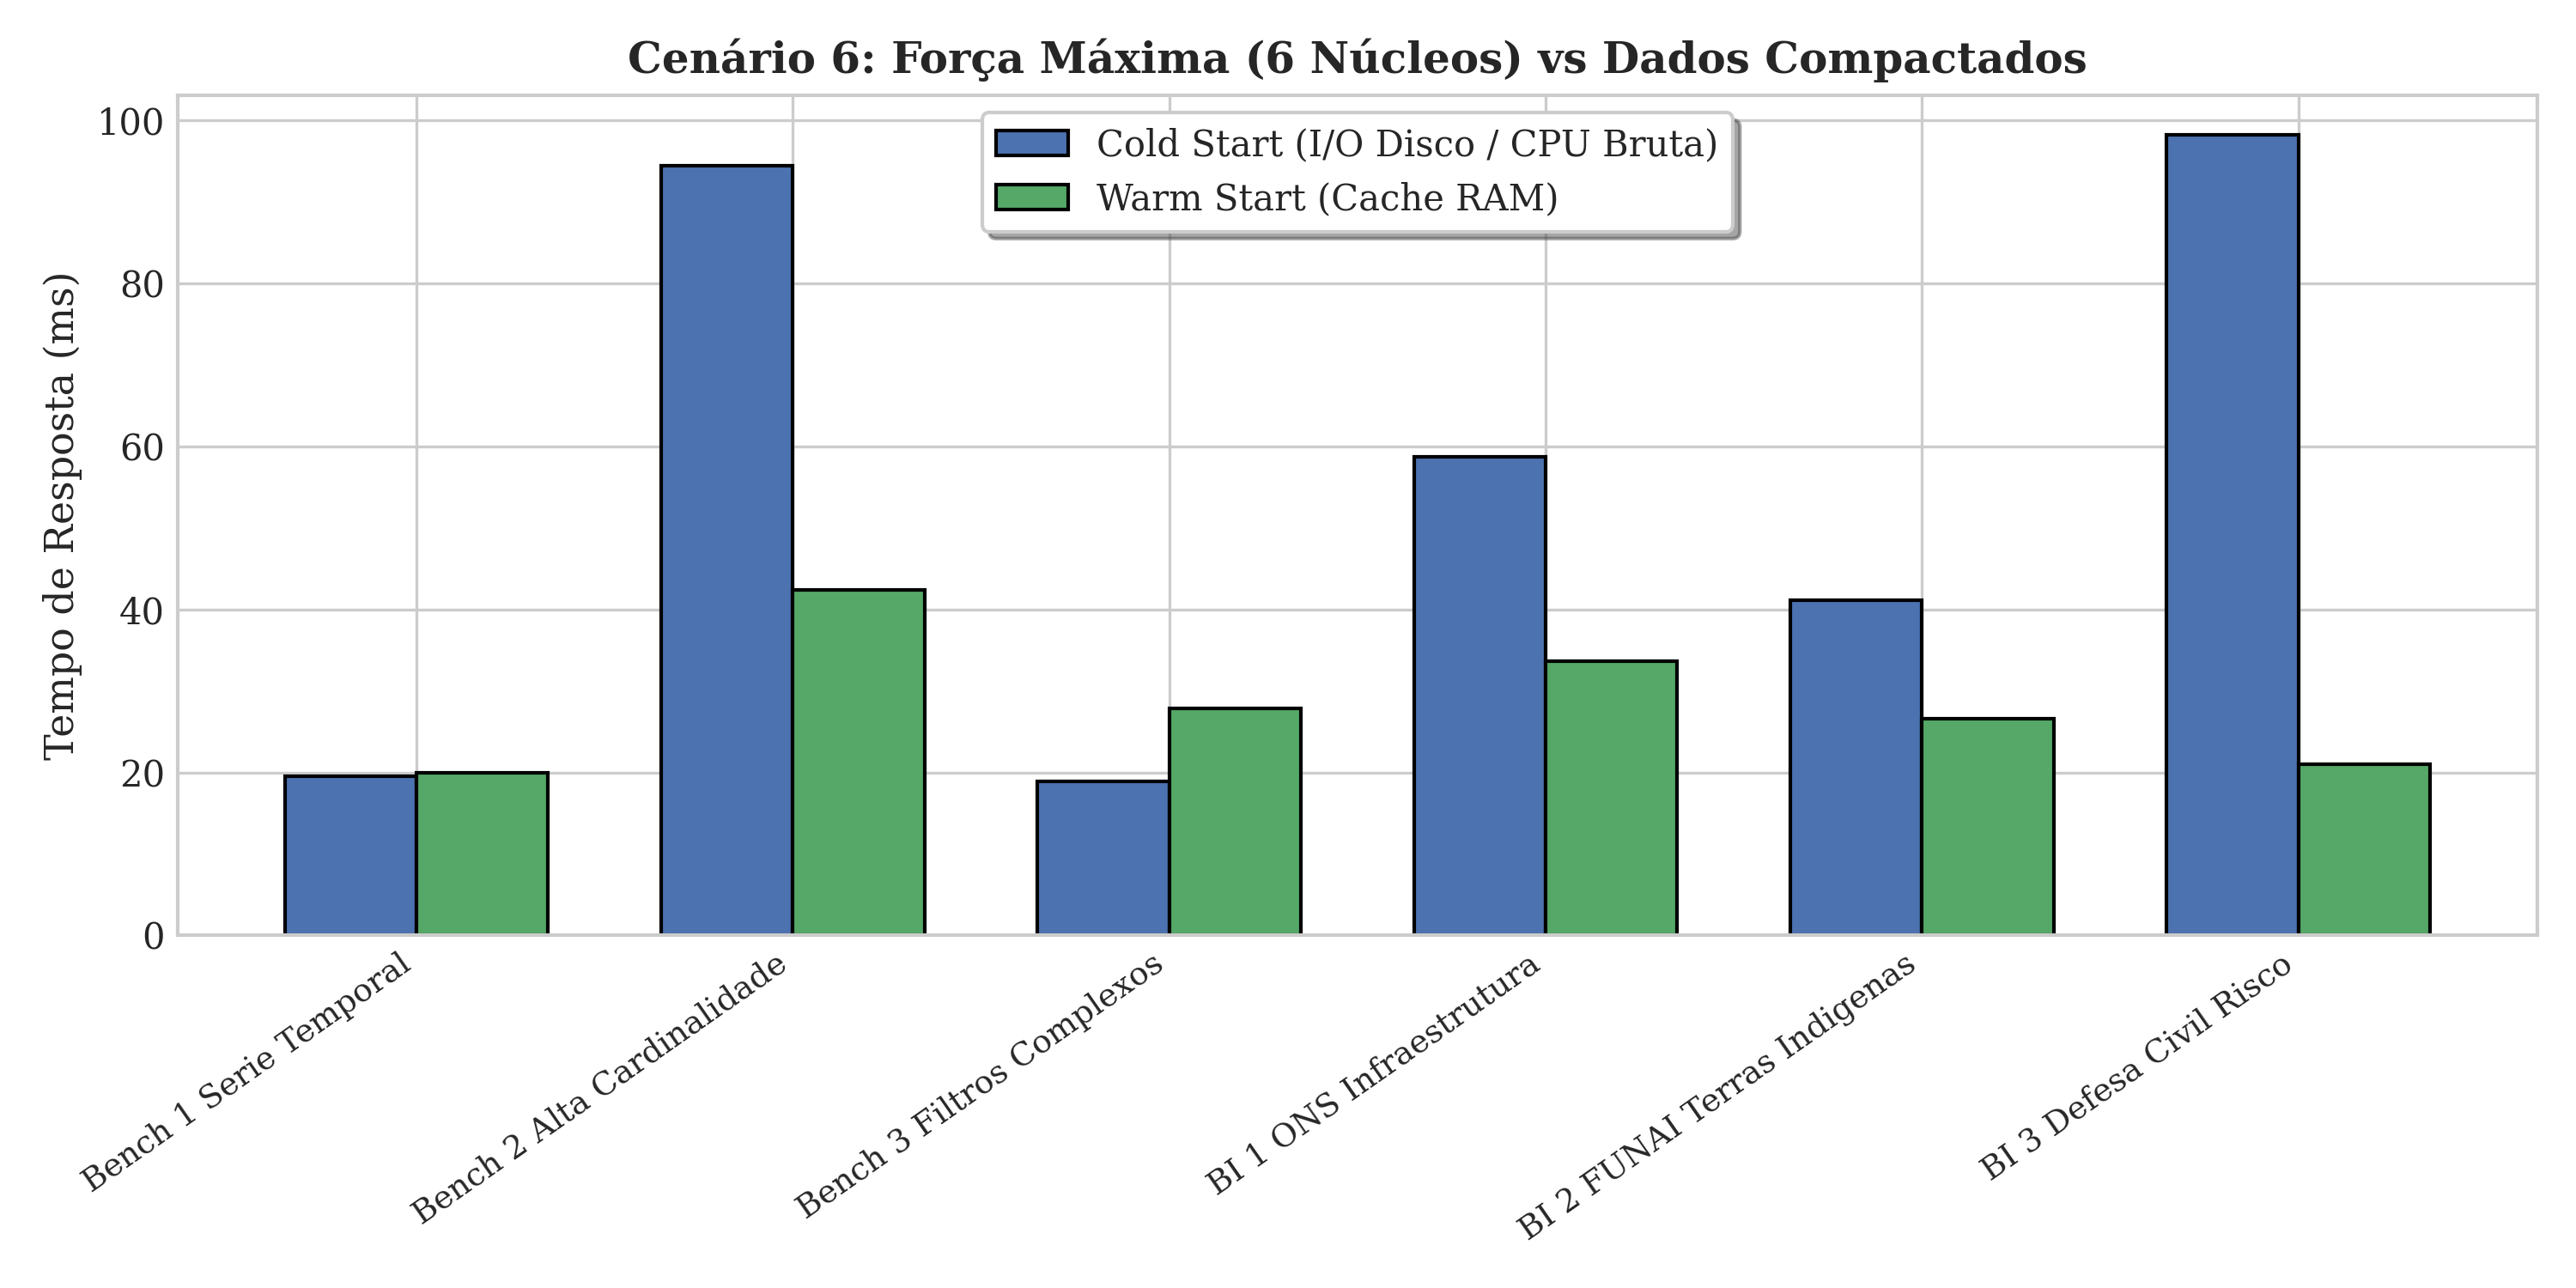
\includegraphics[width=0.9\textwidth]{fig_desemp_cenario6.png}
\caption{A latência bruta atinge seu piso fisiológico, rivalizando com a própria memória.}
\end{figure}

Isto ocorre porque, operando a 18ms, a consulta é mais rápida do que o tempo logístico do nó \textit{Broker} em efetuar o \textit{hash} da requisição HTTP, verificar a integridade da chave no cache e transmitir o binário armazenado. 

\begin{figure}[H]
\centering
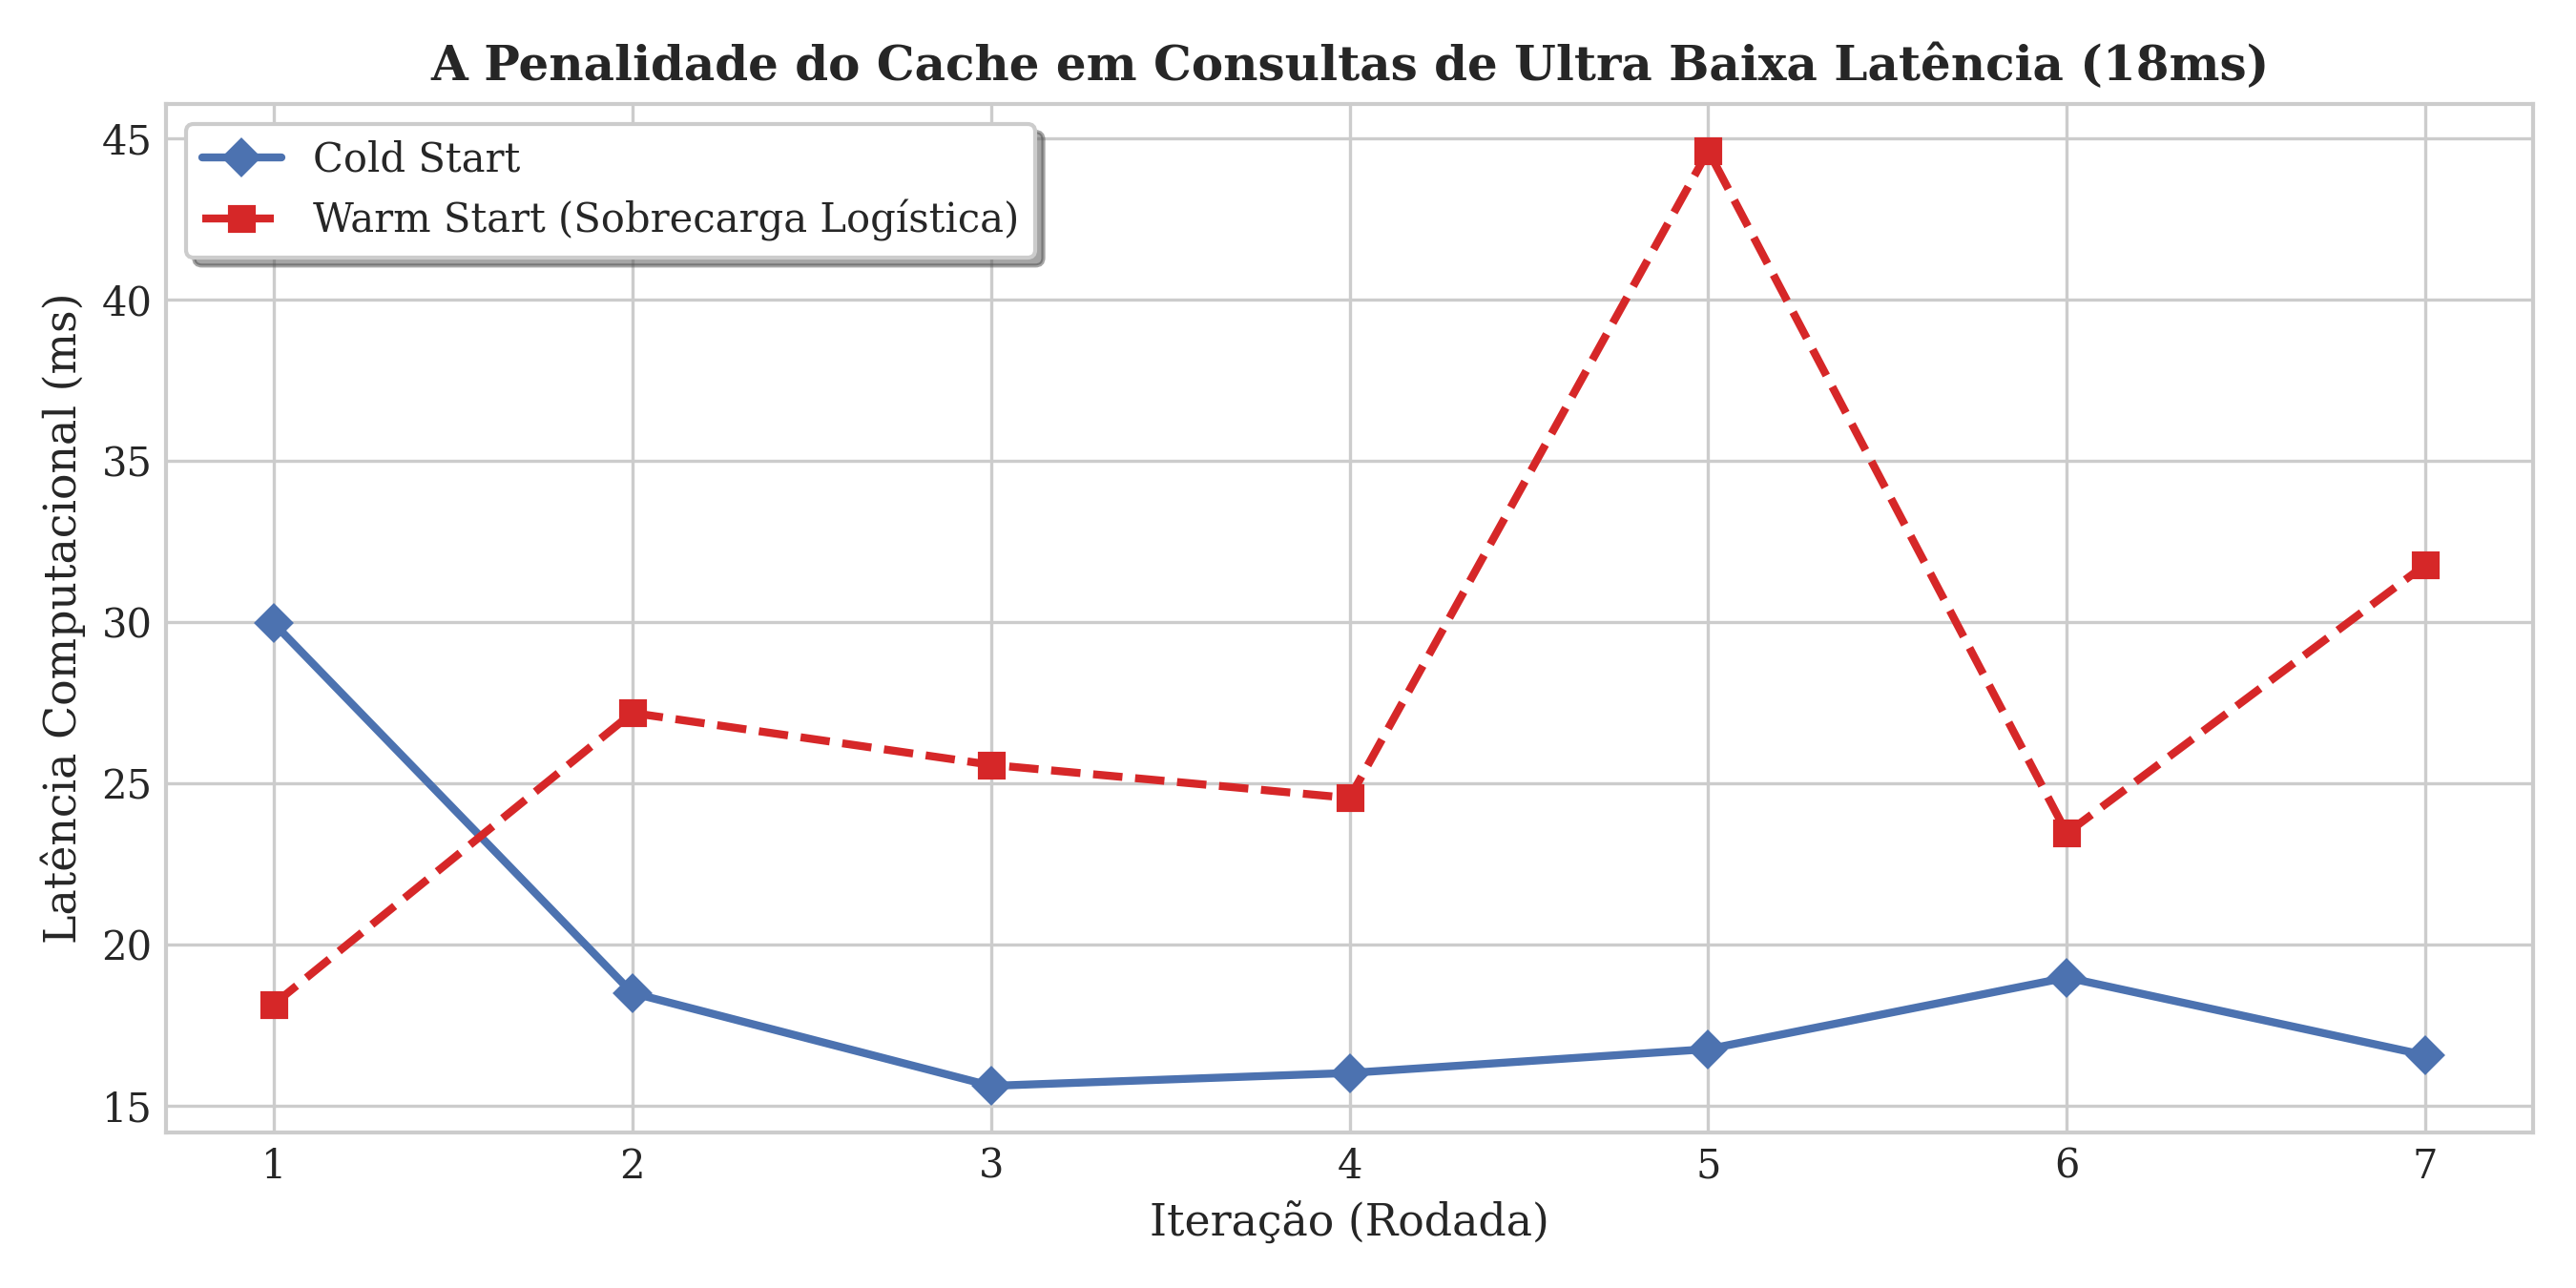
\includegraphics[width=0.8\textwidth]{fig_var_cenario6.png}
\caption{A inversão estrutural: o cache torna-se mais lento que o processamento bruto.}
\end{figure}

\section*{3. Conclusão Final do Projeto}
A bateria de testes comprova que \textbf{escalabilidade vertical possui limites econômicos e matemáticos rígidos}. A diferença de tempo absoluto entre alocar 4 núcleos (Cenário 5) e 6 núcleos (Cenário 6) foi de meros $\sim$20 milissegundos para a maioria das cargas. O grande divisor de águas, responsável por uma aceleração na ordem de $\times40$, foi exclusivamente a disciplina de \textbf{DataOps} (Compactação de Segmentos). A pesquisa conclui que bases analíticas (OLAP) modernas devem priorizar a engenharia de \textit{storage} e compactação sobre o provisionamento desenfreado de CPU.

\end{document}
